\chapter{The Conceptual Model}
\label{chp:concept}

This chapter examines the ways in which retroaction can be applied to event
sourcing. We discuss conceptual considerations and illustrate how 
different architectures can be utilized to enable retroactive capabilities 
of event-sourced applications.

\section{Retroactive Computing}
In order to examine how retroactive capabilities can be utilized in event-sourced 
systems, we explicitly examine event sourcing \emph{in a CQRS context}. As described 
in Chapter~\ref{chp:background}, event sourcing and CQRS form a symbiotic relationship 
which is commonly taken advantage of. By assuming such a style of architecture, we 
can focus on how the event sourcing foundation can be utilized. This is not to say 
that we do not examine other architectures. 
Indeed, in Chapter \ref{chp:chrono} of this thesis we examine if and how the concepts 
described in this (and the succeeding) chapter can be applied to a different 
architecture.  The Chronograph platform is the foundation for this second examination; 
it applies event sourcing in a context which has only few commonalities with the 
traditional CQRS style of architecture.


\section{Conceptual Considerations}
This section provides an overview on key challenges when utilizing 
retroaction in event-sourced systems.
We propose possibilities of how to handle these issues, but do not 
claim to lay out the one true way in which retroactive computing should be 
done in event-sourced systems. We rather aim to illustrate that depending 
on the context of a system, different conceptual choices are best-suited.
We deliberately restrict the context in which we examine retroaction and 
focus on three example scenarios of event-sourced applications with different 
requirements and issues. 
The topic of retroaction is very extensive and appointing these three 
scenarios as cornerstones of our examination provides a guideline and helps 
us illustrate complex issues.

\paragraph{Weather Station Application} 
	In this scenario, sensor readings are fed into the application via commands.
	These commands result in events, which do not possess causal relationships 
	among each other. 
	Based on this data, the application generates statistics and forecasts. 
	The scenario is not complex and poses only few issues for retroaction.
	%
	Examples of retroactive operations in this scenario are the correction of 
	faulty values, the retroactive addition of missing values, and the 
	reconstruction of historic statistics and predictions. 
	Comparing the outcome of different forecast algorithms based on the historic 
	data is another use case. 

\paragraph{Internet of Things Controller} 
	The application manages several independent Internet of Things (IoT) devices. 
	These devices send status information to the controller, which maintains a 
	global view on all devices and issues new commands to them.
	The global view of the controller is based upon the status information which 
	it receives from the devices; commands are issued based on this constructed view.
	As such, this scenario possesses a close coupling between the application and 
	its environment: 
	The system state affects the environment, which in turn affects the system state.
	Retroactive use cases here include the analysis of incidents.
	Not only can incidents be reconstructed, changes to the controlling logic can be 
	simulated as well. Furthermore, the historical application data can be used to
	optimize the control algorithm.

\paragraph{Online Shopping Service} 
	The online shop combines warehousing, order processing, pricing, and accounting. 
	By utilizing retroaction, prices or inventory errors can be corrected retroactively. 
	Simulations of changes to discount algorithms or price calculations can be performed 
	based on past transactions. This scenario is heavily affected by side effects (e.g. 
	sending order confirmations), hidden causalities (e.g. the impact of prices on actual 
	orders), and a strong coupling (e.g. effect of orders on article availability).

\subsection{Command Sourcing}
\begin{figure}
	\centering
	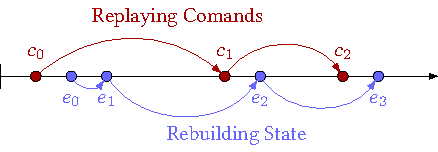
\includegraphics[width=0.6\textwidth]{../illustrations/event-log.pdf}
	\caption{
		When commands and events are sourced, this results in a timeline 
		of commands and subsequently their resulting events.
	}
	\label{fig:event-log}
\end{figure}

In a strict event-sourced system, only events are sourced, but not the commands 
which triggered their creation in the first place. The current state of a 
system derives from this series of events and can at any time be rebuilt by 
applying each event successively again (starting from the first event). 
It is important to note that in such an event replay no commands are invoked, 
since the events are not newly computed. This is opposed to a command replay, 
in which each command is invoked again. 
As a result, the commands may yield the same events or different ones, but the 
events have been newly computed.  
A command replay poses a central issue to retroactive computing: If a command is 
invoked again, side effects might occur again. An event-replay, on the other hand, 
does not trigger any side effects, since only existing events are used to rebuild 
state.

By sourcing commands and events, the retroactive capabilities gain in 
expressiveness and a number of applications are possible, which are not feasible 
in a system which sources only events.
For instance, it is possible to test how a system would have reacted differently,
if a different logic (i.e. a different command processing) had been in place.
In order to evaluate how a different command processing would have affected 
the behavior of a system differently it is necessary (1) to source commands
and (2) for the command processing to be decoupled from the command.
Decoupling the command processing from commands can be modelled by a command
processor component which receives a request to invoke a certain command, executes 
appropriate processing logic, and produces events (Chapter \ref{chp:background}).
One can then use the recorded set of commands and replay them with a different 
processing implementation.
In relation to our three scenarios, commands can be modelled as sensor data 
streamed into the system (weather station, IoT) or as orders and inventory 
updates (online shop).

For the remainder of this thesis, we focus on systems which source commands and 
events. We refer to the log of such systems, the combination of command and event 
log, as the \emph{timeline}.
Figure \ref{fig:event-log} depicts an example of a timeline.
Here, a command in the timeline can result in one or more events. If we write of 
``events'' resulting from a command (as opposed to the singular ``event''), we imply 
that the result could also consist of a single event.

\subsection{Editing the Event Log}
\label{sec:editing-log}
\begin{figure*}
	\centering

	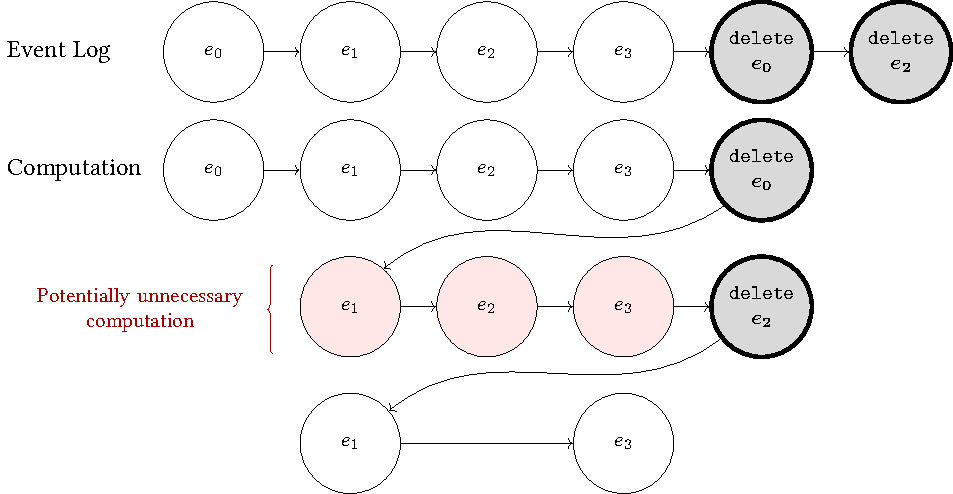
\includegraphics[width=0.8\textwidth]{../illustrations/reversal-events2.pdf}
	\caption{
		This figure depicts a possible course of computation when events 
		are appended to denote retroactive modifications.
	}
	\label{fig:reversal-events}
\end{figure*}

The append-only nature of the event log in event-sourced systems creates a lot 
of the advantages which one usually aims for with an event-sourced architecture 
(see Section \ref{sec:es-cs-benefits} for a detailed explanation).
For retroactive commands, this append-only restriction implies that retroactive 
changes to the event log need to be appended as well. We mentioned Fowler's 
retroactive events \cite{Fowler2005_2} as a mean to apply retroactive changes 
to the event log.
These retroactive events are appended to the event log to denote that the 
effect of a previous event should be revoked by modifying the \emph{current} 
status in a way as if a certain event had never occurred. In the case of the
online shop, a retroactive event which fixes a false inventory update could set 
the inventory stock back to a prior number.
It is important to note that the originally false event remains in the event log.
The usage of these retroactive events is not motivated by retroactive explorations 
of insert or delete modifications to the event log, the intention rather is to 
add fixes to the log. 
Fowler proposes three basic types of retroactive events for this: out of order 
events, rejected events, and incorrect events. 

Retroactive events suit well for typical productive event-sourced systems, in
which it is crucial that events are only ever appended and never deleted or
retroactively injected. Otherwise a lot of the event sourcing characteristics 
(e.g. benefits for scalability, traceability, or the possibility to rebuild
application state at arbitrary points in the timeline) would no longer hold.
The motivation behind the research in this thesis, on the other hand, is to
explore how modifications to the past of a timeline affect the current state 
of a system. Appending reversal events is not an appropriate tool for 
this purpose, since it cannot always be easily calculated how the current
state of the system would differ. 
This calculation would be equivalent to resetting the system to a previous 
state, applying modifications there, and re-playing events (or replaying 
commands) from that point on.
A series of retroactive changes would then lead to expensive and potentially 
unnecessary computations being executed (Figure \ref{fig:reversal-events}).

A contrary possibility to apply retroactive modifications, is to directly edit 
a timeline without appending commands or events to the timeline.
We refer to such retroactive modifications as \emph{retroactive operations}. 
These are the insertion or deletion of commands (or events), as well as the
exchange of command processing logic.
Even though direct editing violates the append-only behavior of the timeline, 
this does not necessarily contradict the principles of an event-sourced system. 
We propose to apply two different views here. By distinguishing between a 
\emph{main timeline} and \emph{branches} of this timeline, we can utilize the 
advantages of both options. 
The main timeline resembles the application itself and retains the append-only 
behavior. It cannot modify its own past. It is though possible to create 
branches of this main timeline.
Branches are copies of a timeline. They were created at a certain time and
contain everything that was in the timeline at that point in time. 
Modifications on them do not affect the original timeline. In contrast to a 
timeline, they possess a direct editing semantics. 
If results from these branches are to be returned into the main timeline, this 
can be done using event sourcing primitives -- by appending events.

This decoupling of ``productive'' system and retroactive explorations already 
prevents obvious issues of retroactive systems: A paradox could emerge once the 
application modifies its own timeline in an inconsistent way. This can happen 
once it introduces a contradiction to the current state into its own past -- e.g. 
by modifying its history in a way that it could never have executed such a 
modification. Moreover, keeping the append-only characteristic for the main 
system flow does not break with benefits of event-sourced architectures for e.g. 
scalability and traceability.
The following example illustrates this issue with a delete operation. For this, 
we assume that a system receives commands which influence and trigger the purchase 
of stock options. 
In the example, we use numbers as unique identifiers for commands (\cmd{c})
and events (\cmd{e}), but this is only for illustration purposes. Events usually 
do not have an incremental identifier.

\begin{lstlisting}[style=styled]
c0: someComputation(): // ...
e0: buyStock = false

c1: newData(...): if (data.price < 100) buyStock = true;
e1: buyStock = true

c2: checkBuying(): if (buyStock = true) buyStock();
e2: boughtStock = true

c3: delete("c1" and "e1"); 
\end{lstlisting}

The resulting timeline looks like this:

\begin{lstlisting}[style=styled]
c0: someComputation(): // ...
e0: buyStock = false

c2: checkBuying(): if (buyStock = true) buyStock();
e2: boughtStock = true

c3: delete("c1" and "e1"); 
\end{lstlisting}

It is no longer clear why stock was bought in the first place. In some corner 
cases, this may get clearer if the command model only possesses one possibility 
which could have triggered \cmd{buyStock()}, but this cannot be generalized.

In the case of insert operations the traceability of a system breaks as well. 
In the following example it can no longer be clearly traced what originally 
triggered the purchase, if an event ``\evt{bar = true}'' is inserted after 
\cmd{e0}. There are certainly means to circumvent this behavior (e.g. saving 
timestamps with events), but this then still works against the append-only 
behavior of the event log.

\begin{lstlisting}[style=styled]
c0: foo = false;
e0: foo = false

c1: if (foo == false || bar == true) buyStock();
e1: boughtStock = true
\end{lstlisting}

If a system applies retroaction only to branches and appends the results from
retroactive computations on branches to the timeline using command/event 
primitives, then it is still possible to trace how certain states of the 
timeline occurred. From our point of view, Fowler's retroactive events are the 
only appropriate mean to apply retroactive operations on the main timeline 
without breaking traceability or the append-only property. Thus, in the case 
of the weather station, they are an appropriate tool to correct faulty values
or retroactively insert later ones.
Branches, on the other hand, fit very well to conduct e.g. experimental 
retroactive analyses and return their result to the application. In the IoT 
scenario this could e.g. be the analyses of an experimental device controller.
For the remainder of this thesis, we focus on the direct editing \emph{of branches}. 
As illustrated, it fits better to the objectives of retroaction in our context. 
Furthermore, we use the term \emph{retroactive queries} when referring to queries
which operate on a branch.

\subsection{Consistency and Validation}
\label{sec:validation}
An implication of directly editing a branch is that whenever a change is 
introduced into the past, these changes affect the subsequent part of the 
branch. Thus, in order to ensure a consistent branch, editing operations 
need to be complemented by further measures.
Otherwise causal violations (i.e. a paradox) could occur when a contradiction 
is introduced into the branch. For example, an excerpt of the online shop's 
event log could look like this:

\begin{lstlisting}[style=styled]
c0: Create Product A, Inventory Stock = 10
e0: Created Product A, Inventory Stock = 10

c1: Order 10 Items of Product A
e1: Ordered 10 Items of Product A
\end{lstlisting}

An example of an illegitimate change to this example would then be to inject 
the event ``\texttt{Ordered 1 Item of Product A}'' between \texttt{e0} and 
\texttt{e1}, since this would result in a negative inventory and depending 
on the domain model a negative inventory might be prohibited. The event 
\texttt{e1} would thus not be consistent with the domain model after this 
particular retroactive modification.
There are a number of options how the consistency of a timeline can be ensured.
In the related work chapter on time travel theory (Chapter \ref{chp:related-work}), 
we already mentioned two possibilities to prevent paradoxes: the usage of 
parallel universes and the self-consistency principle. We now describe how the 
self-consistency principle can be applied to retroaction in event-sourced systems:

\paragraph{Removal of Causally Dependent Events}
Causally dependent events can be recursively removed, by forward deleting all 
events which have been directly or indirectly influenced by a specified event. 
After this cleanup process, all consequences of an event have been removed from 
the timeline.
In order to realize this, causal dependencies between events need to be recorded. 
In the online shop scenario, this can be used to prevent paradoxes. When e.g. an 
event \texttt{PlacedOrder} is removed from the timeline, all causally dependent 
events (e.g. \texttt{ParcelShipped}) can automatically be removed as well.
The concept of tracing causal dependencies among events will be detailed 
in the next section. Limitations of this approach are discussed there as well.

\paragraph{Replay of Causally Dependent Events}
A similar approach to ensure consistency is to recompute all events from the
point of the retroactive change on. 
This can be achieved by reprocessing the commands belonging to these events,
which ensures that succeeding events were computed with these retroactive 
changes taken into account. Transferred to time travelling, this means that 
everything happens again, though it might happen differently this time.
This possibility requires capturing causal dependencies as well. 
Its limitations will also be detailed in the next section.

\paragraph{Validation}
The self-consistency principle from time travel theory can also be applied to 
restrain the possibilities of retroactive modifications.
Invariants and pre-/postconditions are possibilities to validate the timeline 
and ensure its consistency. 
If the validation of a retroactive modification fails, this indicates that the 
timeline would no longer be consistent and the modifications thus are not 
allowed. Invariants fit well with the DDD approach of describing a domain 
model and the constraints within it. 
In the online shop, the invariant could describe domain-specific constraints 
(e.g. that product stock has to be a positive number) and event dependencies
(e.g. that in a shopping cart, \texttt{ProductRemoved} events need a foregoing 
\texttt{ProductAdded} event).
%
The challenge with validation conditions is that they can only be checked
\emph{after} the execution of a command. Only then it is clear in which events 
the command results.
If the validation succeeds, the command and event can be appended to the timeline.
If it fails, appending the command and event to the timeline can just be discarded. 
The state of the overall system then remains unchanged. But these validation 
mechanisms pose a challenge for a command yielding side effects. Then discarding 
the command and event from appending is not enough, since the side effects have 
already occurred.
This issue and a possible solution is discussed in Section \ref{subsec:validation}.

\ \\
It can also be appropriate not to constrain modifications to the timeline at all. 
Inconsistent manipulations of the past might even be a fully intended effect.
%
A use case for this is to define a certain application state as a desired target 
state. As a next step, the application's past is modified until the target state 
is reached. This process yields the necessary retroactive modifications as a result.
Thus, constraining the set of possible operations on the timeline by imposing 
validation conditions and constraints might -- depending on the context -- even 
weaken the retroactive capabilities.
An expressive concept can allow to specify the validation behavior when manipulating 
the timeline: validate the timeline for consistency (e.g. by supplying an invariant 
with the intended modification) or execute the modifications with full knowledge 
of possible inconsistencies.


\subsection{Tracing Causal Dependencies}
\label{sec:dependent}

With each operation, which modifies the past of a timeline and is not append-only,
a nontrivial problem emerges:
The state of the system from this point on might no longer be correct, since the 
reprocessed commands could yield different events. 
Thus, the succeeding commands would have had a different premise for their 
execution and they might have yielded different events as a result. Thus 
succeeding events might be causally dependent on prior events. 
But it is not sufficient to only take these \emph{directly} affected events
into account.
Commands or events which have \emph{indirectly} built on these direct events, 
may then have had a different premise as well. 
This trace of causal dependencies affects events which are directly and indirectly 
affected by a modification. Mathematically spoken, these are the events in the 
\emph{transitive closure} of the modified event.
In the previous section, we described the concept of self-consistency for
a timeline by either recursively recomputing causally dependent events or by 
recursively removing them.
This recursive process can lead to a cascade of rippling replays (or removals) 
which work through the timeline.

The concept which we just described lacks the information \emph{how} it is
possible to trace which commands are affected by a state change. This trace 
can be described using event sourcing primitives: For each command it needs 
to be clear what information it used to get to its result, i.e. upon which 
events it built to calculate the events which it yielded as an output.
This approach enables the creation of a trace for each command, tracing which 
commands are affected by a retroactive modification, and recursively recompute 
them.
A concrete algorithm for this is detailed in Section \ref{sec:events-as-statem}.
A limitation of this process is that hidden causalities outside of a system might 
exist (e.g. through side effects). It is not possible to capture those and 
thus not all commands necessary might be replayed. This limitation is described 
further in \mbox{Section \ref{sec:hidden}.}

We see multiple possibilities how the information upon which events the commands 
have built can be recorded. One possibility is for developers to manually 
annotate this information and e.g. return it from the command. Another option is 
the usage of getter and setter methods which record access to objects.
In some cases, this annotation could also be done automatically through 
an underlying platform (e.g. utilizing source code analysis).

\subsection{Side Effects}
\label{sec:side-effects}
Dealing with side effects is an important and nontrivial issue, which needs
to be solved in order to fully utilize the retroactive capabilities of 
event-sourced systems. Certainly one can prohibit applications to yield any 
side effects, but as other authors \cite{Jones2001, Salkeld2011} have 
recognized, many interesting applications are only possible because of side 
effects (e.g. input/output or networking).

In the context of our scenarios, the weather station application possesses no 
side effects. The application only gets data into the system via commands and 
its interaction with the outside system is limited. 
The IoT scenario and the online shop, on the other hand, possess a number of 
side effect afflicted operations: sending order confirmations to customers, 
validating payment details using external services, or issuing control commands 
to devices, for example. When examined closer, it becomes clear that the 
problem has two parts to it: \emph{validation and control}.
We examine these two issues subsequently.

\subsubsection{Validation of Side Effect Afflicted Commands}
\label{subsec:validation}
The timeline can only be validated for consistency after a -- possibly side 
effect afflicted -- command has been executed. Only then it becomes clear, in 
which events the command results. If this validation fails, the event is not 
persisted and the question arises how the already invoked side effects within 
the command can be revoked. For purely reading side effects this is not a 
problem, since they do not mutate state outside of the system. But for state 
mutating side effects this problem needs to be handled.
One could see the solution in adding adding undo (or rollback) commands, which 
would reverse these side effects. But this idea hits upon problems as soon as 
the side effect is irreversible -- which is the case with e.g. order confirmations 
(online shop) or actions sent to devices outside of the system (IoT).
A better possibility is to delay the execution of state mutating side effects
until the result of the command has been validated and it is certain that the 
resulting events are appended to the timeline.
This approach has limitations as well, as soon as e.g. internal logic depends 
on their prior invocation.
But it at least is a possibility to validate side effect afflicted commands.

\subsubsection{Controlling Side Effects in Replays}
\label{sec:replaying-se}
The second challenge concerns the question how the behavior of side effects 
can be controlled when a side effect afflicted command is replayed.
%
When state is rebuild, this can be done by examining the series of events
in the timeline (Figure~\ref{fig:event-log}).
There are no side effects from such an event replay, since events denote only 
changes in state and their replay does not trigger their recomputation. 
But side effects can be caused by replaying (i.e. reprocessing) commands. 
A problem here is that one cannot find a general rule of how to handle
side effects in a replay. If commands are replayed with a purely
experimental intention, it can be undesirable to have some of the side effects 
triggered again.
An online shop which replays customer interactions on the new backend for pure 
testing purposes will not want to have order confirmations sent out again.
Console output or logging facilities, on the other hand, might be desirable
side effects of such a replay for testing purposes.

Handling this ambiguity of side effects when working retroactively is an issue 
which Salkeld et al. \cite{Salkeld2011} have described: 
``We are continuing to investigate the best approach for managing side effects. 
It is unclear how to rigorously permit intentional, safe side effects in 
retroactive advice [\dots]''.
Since the treatment of side effects is highly domain and context dependent
it needs to be possible to specify how a side effect should behave when it is 
replayed. There are two behaviors which we aim for:

\begin{enumerate}
	\item Reinvoke them and use the new result for the further processing
	(e.g. fetching a web page again).
	\item Suppress their new invocation and reuse the result from their 
	first invocation (e.g. reusing a generated random number or reusing 
	the result from a prior dispatching of a mail message, instead of sending 
	it again).
\end{enumerate}

One could see the solution in adding the possibility for the command processing
to know if it is currently replayed.
If the command processing can be exchanged before a replay takes place, this
would enable developers to specify how specific side effects within a
command should be handled.
This would solve some problems with side effects, by providing some form of 
control over them. But it does not solve all issues with side effects.
For example, a command might have had a side effect which returned a value.
In a command replay scenario it might be desirable for the side effect to 
return the same value as it did when executed for the first time. 
For example, in the online shop scenario a \texttt{PlaceOrder} command could 
have an internal credit card validation logic which uses an online service.
If one were to replay the commands in the timeline, in order to find out if an 
optimized warehousing algorithm would have reacted better to inventory changes, 
it would be desirable to have the side effect return the same validation 
results as it did in the ``original'' recording. Otherwise it would be hard 
to compare the results of both algorithms. 
For this purpose, the result of the validation requests needs to be recorded
somehow.  Enabling commands to know if they are currently replayed does not 
solve this issue.
Additionally, for commands to know if they are currently replayed contradicts
a deterministic behavior of replays. A replay could then yield entirely 
different results, each time it is conducted. 
%
In order to gain full control over the behavior of side effects in replays, it 
is necessary to record the result of side effect afflicted operations.

A concept proposed by Fowler, as a mean to handle side effects in event-sourced 
systems, is the usage of gateways \cite{Fowler2005}. He describes gateways as 
special objects which encapsulate side effect operations \cite[p.~466]{Fowler2002}. 
The behavior of these gateways in a replay is defined by the application which 
triggers the replay. An issue here is that it is unclear how gateways should 
record the operations which pass through them. 
Additionally, gateways do not suit well for the concept of branches: they would
need special attention and handling when creating or replaying branches, since 
they do not tie in with the common event sourcing primitives. 

Before we describe a possibility for handling these issues further, let us first 
examine what types of side effects can occur in an event-sourced system. There 
are three kinds of side effects which may occur in commands in event-sourced 
systems (Fowler uses a similar categorization \cite{Fowler2005}):

\begin{itemize} 
	\item \emph{External Query}: Reading data by interacting with an outside 
	system. In the online shop scenario this can e.g. be the reading of a 
	currency exchange rate from an online service.
	%, as a mean to display shop prices in alternate currencies.

	\item \emph{External Command}: Mutating data in an outside system.
	In the IoT scenario, the controller sends commands to devices outside
	of the system.
	These commands are irrevocable, as soon as they leave the system.
	Sent order confirmations in the online shop are a further example.

	\item \emph{External Query + Command}: The combination of both.
	An example is an external payment service used by an online
	shop. The shop could request a payment, as part of a
	process to place an order. A notification could indicate if the
	payment was successful or failed.
\end{itemize}

For external queries in a replay scenario, it should be possible to specify if they 
should either be executed again or if the result which was originally returned
should be reused. Reusing an already existing result implies that the new invocation 
is skipped.
%
External commands are supposed to be strictly state mutating and to not return any 
state. It should be possible to specify if they should either be executed again or 
not be executed again (skipped). It should also be possible to handle the 
combination of both by specifying re-executions or the reusage of prior results.

To achieve this, we propose an idea which ties in with the characteristics of an 
event-sourced system -- namely the event log and sourcing commands and events for 
restoring state or reprocessing commands. The concept of \emph{partial replays}
enables us to control the behavior of side effect afflicted commands in a
replay. Partial replays form a combination of event and command replay.
Here it is possible to specify the behavior of individual commands and events in 
a replay by controlling:

\begin{enumerate}
	\item If a persisted event should be used instead of invoking the command again.
	\item If a command should be re-processed.
\end{enumerate}

\begin{figure}
	\centering
	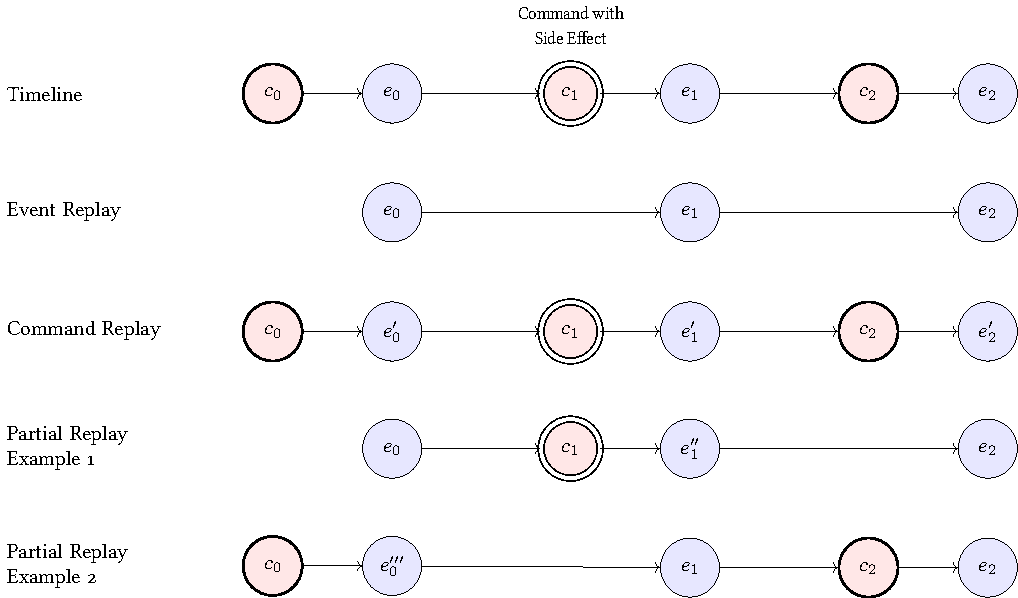
\includegraphics[width=1.0\textwidth]{../illustrations/partial-replay2.pdf}
	\caption{
		The figure depicts different possibilities for replays of a timeline.
		In an event replay, state is rebuilt based solely on events. 
		In a command replay, each command is invoked again and events are 
		newly computed. % (hence the ``$'$'' in the event labels).
		In a partial replay, it is possible to control which commands are re-executed.
		In ``Example 1'', the side effect afflicted command is re-executed.  
		In \mbox{``Example 2''}, the side effect afflicted command is not executed again, 
		instead the event from the last invocation is reused. 
	}
	\label{fig:partial-replay}
\end{figure}

Different replay sequences are depicted in Figure \ref{fig:partial-replay}.
The figure though only depicts small sequences. A problem which becomes visible 
in larger sequences, is that through the reprocessing of a command, a different 
event (or multiple different events) than in the original computation may be 
computed. The state of the system from this point on would then be different. 
Thus, subsequent commands may have executed a different logic, which possibly 
would have yielded other events.
Section \ref{sec:validation} discussed two solutions to this problem: 
recomputing causally dependent events as well or removing causally dependent 
events. 

We propose to leave control over how fine-grained side effect afflicted 
commands can be controlled to the programmers and domain experts. 
We therefore propose to split side effect afflicted commands into multiple 
commands, with the side effects being isolated in individual side effect 
afflicted commands with few logic.
In partial replays, all three types of side effects result in command-events 
pairs with no further distinction if they have a reading or writing side effect, 
or none at all.
Side effects then are encapsulated in individual commands and events. This 
concept enables us to view side effects as isolated and thus we can control
their individual behavior in a replay. It is then possible to e.g. specify 
that results of a command \cmd{SendOrderConfirmation()} should always be 
reused. Thus the order confirmation side effect will not be invoked again. 
This also enables us to specify that e.g. a command \cmd{FetchStockPrice()} 
is invoked again. As a consequence, all events which are causally dependent 
on this result can be reprocessed as well (i.e.  the respective commands are 
reinvoked). This can be achieved by examining the trace of causalities among 
events as described in Section~\ref{sec:dependent}.
%
But this concept implicates that it needs to be possible to split commands.
Three possibilities how this can be achieved are:

\begin{enumerate}
\item For the application, which issues commands to the API, to split a 
command into an ordered series of multiple, smaller commands. These commands 
are issued sequentially. Each command in the series needs to complete, before 
the subsequent command is issued.

\item For the API to provide a thin logic layer which splits an incoming 
command into multiple internal commands which are invoked sequentially, 
one after another.

\item For the command processor to invoke other commands during the processing 
of a command.
\end{enumerate}


The implication of (3) is that the definition of the timeline as a series of 
atomic command and succeeding affiliated events would break up. Instead the 
timeline would consist of nested series' of commands and their respective events: 

\begin{center}
$(command_a\rightarrow(command_b\rightarrow{}event_b)\rightarrow{}event_a)$
\end{center}

Such nested series' break with the event sourcing primitives of pairs of commands 
and event(s). We thus do not consider (3) further. The requirements for (1) and 
(2) are:


\begin{itemize}
\item When executing a series of commands, this series is fixed. The component 
which issues the individual commands (the API or the application) does not 
deviate from this series. No further logic is executed during the execution of 
the series. Otherwise the determinism of replays is endangered, since this 
``logic layer'' would not be persisted in the timeline and could not be taken 
into account in replays. Thus, replays might not perform the operation as it 
would have really occurred.

\item Each command is persisted in the timeline, independent of its success or 
failure. This enables later replays with possibly different results.

\item The execution of this series is done sequentially (or in a causally 
equivalent, serializable order). Each command has to finish its execution 
before the subsequent command in the series is invoked. After each command 
returns, it needs to be checked if the command succeeded. If it did, the 
command and the resulting event are persisted to the timeline and the next 
command in the series is invoked. If the command failed, the commands in the 
series will not be invoked further. But the commands will still be persisted 
to the timeline, in order to enable later command replays.
\end{itemize}

Without those requirements, a causally equivalent (i.e. deterministic) replay 
of persisted commands in the timeline is no longer possible. This issue is 
detailed further in Section \ref{sec:determinism}.

We now describe a brief example of this concept. Consider a hypothetical 
command \texttt{ValidateCreditcard} as part of the logic behind the online 
shop scenario. The command authorizes a credit card using an external service, 
which it accesses over a web service:

\begin{lstlisting}[style=styled]
CommandModel.process("ValidateCreditcard"){
	/* side effect */
	var validation = fetch("https://.../check-card", ...);
	if (validation == true) {
		return Event("OrderPlaced");
	} else {
		return Event("OrderCanceled");
	}
}
\end{lstlisting}

This command can be broken into two succeeding commands, 
\texttt{ValidateCreditcard} and \texttt{PlaceOrder}.
The \texttt{ValidateCreditcard} command executes the side effect
afflicted operation. This results in an event being persisted and the
side effect effectively becoming part of the state of the system: 

\begin{lstlisting}[style=styled]
c0: ValidateCreditcard()
e0: ValidationSuccessful

c1: PlaceOrder()
e1: OrderPlaced
\end{lstlisting}

The \texttt{PlaceOrder} command can then execute logic based on the fetched 
validation result. In a replay it can be controlled if the side effect should 
be executed again (i.e. the command reprocessed) or if the already persisted 
stock price should be used.

The advantage of such a series of (possibly side effect afflicted) commands
and their events, over the concept of gateways is that they specify clearly 
how the results of side effects are recorded and how their behavior can be 
controlled when a replay is executed. 
Also this concept ties in with event-sourced primitives: commands, events, 
and the timeline. This comes in helpful when we use the concept of branches 
on the timeline, since we do not have to pay special considerations to gateways 
and their behavior when branching. As detailed earlier, this splitting can be 
done by the API or by the application. 
As long as the component adheres to the described requirements, a deterministic 
replay is possible.

\subsection{Separated Query and Command Model}
\label{sec:issues-ec}
When retroactive explorations are conducted, the goal usually is to determine
\emph{what} the current state would be \emph{if} the past would have differed.
Such \emph{what-if questions} typically consist of a similar sequence of actions:
a series of operations on the timeline and a concluding query (or multiple queries). 
An example of such a series is:

\begin{enumerate}
	\item \emph{Branch} timeline at a certain point in the past.
	\item \emph{Insert} an event at a certain point in the past of the newly created branch.
	\item \emph{Query} current state of the branch.
\end{enumerate}

What-if questions are hard to realize in a standard CQRS architecture, since 
they require to first execute a series of operations (in commands), before a 
subsequent query can be deposed. 
A separated command and query model with an eventually consistent semantics 
works against such a causally dependent series of commands and queries 
(Chapter \ref{chp:background}).
Without further measures, an application cannot safely assume that the branch 
and its modifications have already been replicated to the query model(s). 
Because of this eventually consistent behavior, it is entirely possible for an 
application to address a query model where not all what-if modifications have 
yet been applied to a branch.
As described in Section \ref{sec:cqrs}, an eventually consistent behavior can 
be seen as a positive artifact of a CQRS architecture.
%
For what-if questions, however, this behavior is disadvantageous, since a 
causally ordered behavior fits better to series' of causally dependent 
operations and queries.
A possibility to address this, is to mitigate the eventually consistent
behavior and delay the fulfillment of queries until the query model is 
updated to a certain version number (a concept used for conditional requests 
in Eventuate\footnote[1]{\href{https://rbmhtechnology.github.io/eventuate/user\-guide.html\#conditional\-requests}{https://rbmhtechnology.github.io/eventuate/user\-guide.html\#conditional\-requests}}).
Another option is to dissolve the model segregation for retroactive operations
and retroactive queries, so that they operate on the same model. 
Causality can then be enforced through the model.
%
A separated retroactive model for retroactive operations and queries offers 
the same benefits as a separated model for application commands and queries: 
individual optimization of each model and the creation of applications with 
inherent eventual consistency in mind.
On the other hand, what-if questions are easier for developers to write, 
if retroactive operations and retroactive queries can be issued causally 
dependent. Developers then do not have to take on the task of ensuring that
queries are only issued, once all retroactive operations have been applied.

\section{Constraints and Limitations of Re\-tro\-action}
\label{sec:cons}
Before we address retroactive architectures further, limitations and constraints 
of retroaction are described in this section. 
The degree to which they apply depends on the actual context of an application.
We do not claim to have solutions for them, they should rather point out the 
limitations of retroaction.

\subsection{Hidden Causalities}
\label{sec:hidden}
In an ideal scenario, no hidden causalities exist in an event-sourced system. 
Thus, when a retroactive change is made to the timeline and a subsequent replay 
is conducted, the outcome is exactly as it would have been if the change had 
originally been in place.
But this ideal scenario is not the case for many systems, as they have some 
coupling to the real world or to other systems.
A danger in the informative value of retroaction lies in hidden (i.e.  untracked) 
causalities of events. 
One event may influence -- directly or indirectly -- the occurrence of subsequent 
events. This is even more problematic if these causalities occur outside of the 
event-sourced system, since they then cannot be tracked.
%
These hidden causalities might weaken the informative value which can be derived 
from the results of retroactive changes. 

To illustrate this on the online shop scenario: The retroactive manipulation of 
the inventory could result in only three car tires being available for purchase. 
This would affect existing car tire order commands in the timeline, since most 
customers would probably only have issued an order if \emph{four} tires had been 
available.
The issue can get even more complex. Maybe there were only three tires in
the inventory all along and through retroactive changes there are now four.
A customer might have taken this opportunity to place an order of four tires. 
On the other hand, a car dealer might have ordered four tires with the
intention of supplying them as spare tires to four different cars, one for each. 
Ordering three tires would have still been fine then. Without knowledge about 
these causalities in the real-world, the system cannot distinguish these cases.
The influence of prices on placed orders is a similar issue.
Thus, caution should be exercised when deriving informative value from 
retroactive results. One should at least take domain knowledge and the
possibility of causalities outside of the system into account. 

These issues are smaller, when an outside system does not further process the 
results of queries. Furthermore, an outside system should not save any state 
based on the result of queries. This can otherwise lead to a (possibly outdated) 
copy of the data outside the system. 
If the outside system makes decisions based on a copy of the data, the 
informative value and expressiveness of retroaction is heavily reduced. This 
issue is especially relevant when the event-sourced system is used as a 
component within a larger system. Such shadow state caches in the application 
are discouraged. 
Hidden causalities can also occur through side effects. These effects take 
place in an outside world and their behavior may be influenced by factors 
outside the scope of the event-sourced system.

\subsection{Causality Violations}
\label{sec:causality-violations}
A further danger of retroaction lies in retroactively induced causality violations, 
such as paradoxes or causal loops. Causality violations occur when we observe an 
effect before its cause. In Section \ref{sec:time-travel-theory}, we have 
described temporal paradoxes where scenarios contain their own negation 
(grandfather paradox). In event-sourced systems, a logical paradox can e.g. 
emerge once an object removes its own producer at a point before it was created.
We have described the emergence of domain model contradicting paradoxes
in the previous section (e.g. placing orders when an item is out of stock). 
%
Another problem of retrocausality concerns causal loops. Causal loops emerge 
when one event is cause for another event, which is a retroactive cause for the 
first event. Without further measures, it can then no longer be determined 
which event was the initial cause. If not handled properly this can break the 
traceability (audit log) of event-sourced systems and when computed can lead to 
infinite loops.  Figure \ref{fig:causal-loop} depicts an example of a causal loop.

These issues are a direct consequence of breaking with the append-only behavior 
of the timeline -- they emerge when the own past is modified. Issues of 
retrocausality limit the possibilities of retroaction and can be source for a 
number of problems. Nevertheless, the possibilities of retroaction can enable 
powerful retroactive capabilities and there are options to limit the impact of 
these issues.
Obvious issues of retroaction can already be prevented by 
\emph{allowing retroactive modifications only on branches of the own timeline}.
This resembles the many-worlds interpretation from time travel theory.
Instead of a single timeline, retroactive modifications yield a new, parallel, 
universe. In the context of retroaction in event-sourced systems, we proposed 
to keep the append-only semantics for the main timeline and feed results from 
retroaction back using commands/events (Section \ref{sec:editing-log}). This 
also complements event sourcing characteristics of traceability and scalability, 
which emerge from an append-only restriction.

\begin{figure}
        \centering
        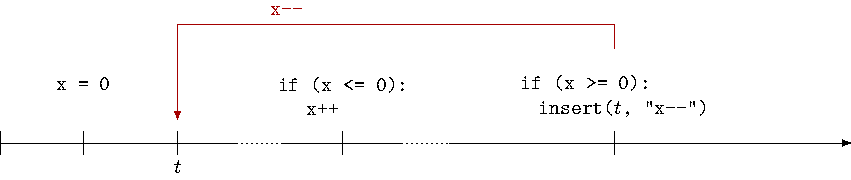
\includegraphics[width=1.0\textwidth]{../illustrations/causal-loop.pdf}

        \caption{
                A causal loop is caused when one event is cause for
                another event, which itself is cause for the first event.
        }
        \label{fig:causal-loop}
\end{figure}

\subsection{Command Semantics}
\label{sec:command-semantics}
When a command has an effect independent of the current state of the system, 
this can have an annihilating effect on retroactive modifications. For example, 
a command \texttt{EmptyShoppingCart} might remove all products from the 
shopping cart. 
Thus, the effects of a retroactively injected command \texttt{AddProductToCart} 
prior to an \texttt{EmptyShoppingCart} command will be overwritten.  
This can lead to unintended reversals of retroaction. This is not necessarily 
a limitation of retroaction, but it can have an unintended limiting effect if 
not taken into account.

\subsection{Causal Equivalence of Replays}
\label{sec:determinism}
In terms of performance, it can be desirable to optimize a command replay 
(using e.g. parallelization in threads or distributed processing). But this 
cannot be achieved trivially by e.g. arbitrarily distributing the command 
processing among threads.
Due to differences in e.g. thread scheduling or network transmission times, 
a replay could then result in a non-deterministic order of processing. 
If the persisted order is deviated from in a replay, the resulting events can 
break the deterministic cause of subsequent events.
Thus, an entirely different application state may emerge each time a replay 
is conducted.
%
To illustrate this on the online shop scenario: If \cmd{PlaceOrder} commands 
are issued in a different order, items in the replay could at different times 
be out of stock instead of available.
Orders which have previously been executed successfully could then suddenly 
fail in a replay, due to a different order of processing. 

A causally equivalent replay also makes it feasible to compare the impact of 
different command processing implementations. For this, commands are replayed 
in a serializable order with a different implementation.
The results can then be compared against each other.
In a non-deterministic replay, on the other hand, unintended variations in e.g. 
processor utilization could as well be responsible for the difference in the 
outcome.

Thus, an event-sourced platform applying CQRS and supporting retroactive 
computing capabilities needs to either (1) provide the guarantee of determinism 
for replays by issuing commands in a serializable order or (2) consciously 
decide to break determinism to gain a better replay performance.  
This decision depends on the context of the application and either behavior
can be desirable.

\subsection{Performance}
\label{sec:perf}
As examined in Section \ref{sec:validation}, the validation of a retroactive 
modification can require checking the foregoing and subsequent timeline 
from the point of the modification for consistency. Removing or recomputing 
direct and indirect causally dependent events might be further performance 
issue. Thus, separating retroactive computations on branches from the 
computations of the live system, on the main timeline might even become necessary. 
%
When retroactive computations are decoupled in a separate, asynchronous environment, 
the main timeline might advance whilst retroactive computations are conducted. 
When computations are expensive and take hours, days, or even weeks, both
systems might diverge and the computed results might no longer be relevant to the 
live system.
Hence, performance issues can have a limiting effect on the value of retroaction and 
it can be important for retroactive computations to be efficiently computable.

\section{Retroaction-enabled Architectures}
\label{sec:arch}
In this section, we examine two contrasting possibilities how retroaction can be 
integrated in an event-sourced architecture following CQRS: 
(1) as a separate component with no modifications to the original architecture 
(i.e.  as a plug-in) or (2) designed right into the architecture (i.e. unified).
This is not to say that these are the only two possibilities. In fact, there 
are a lot of possibilities how this can be achieved, but we focus on two 
outstanding possibilities. 

\begin{figure*}[!t]
	\centering
	%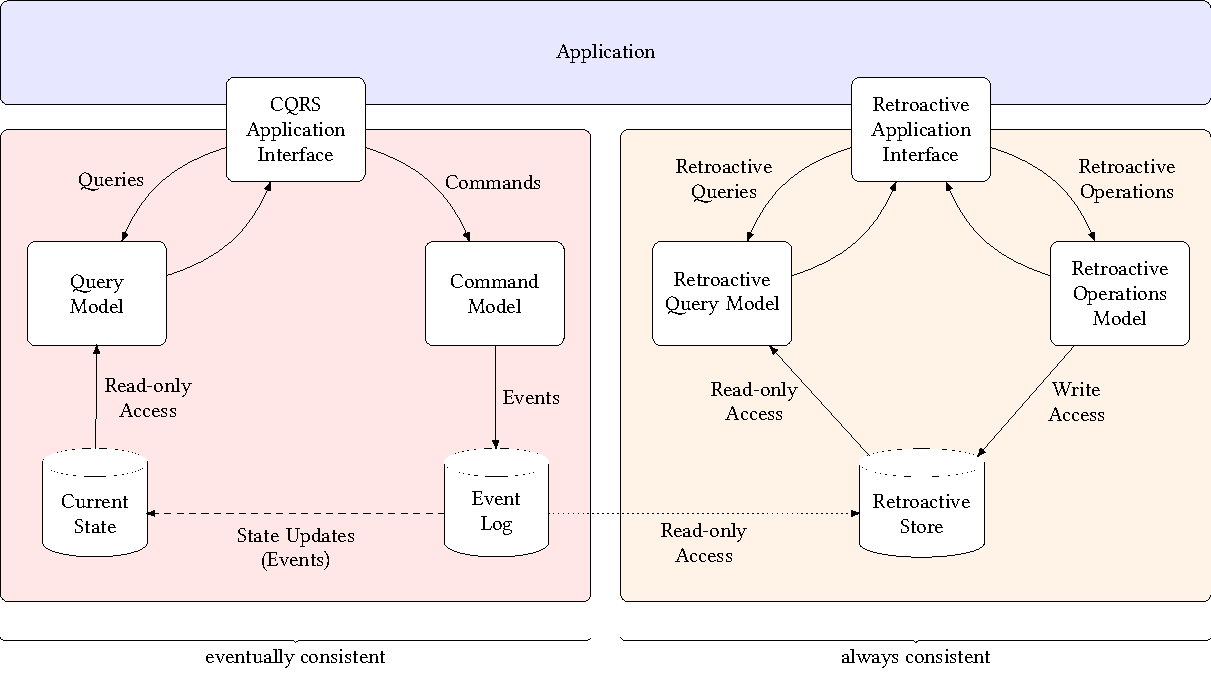
\includegraphics[width=1.0\textwidth]{../illustrations/cqrs-focus-separate.pdf}
	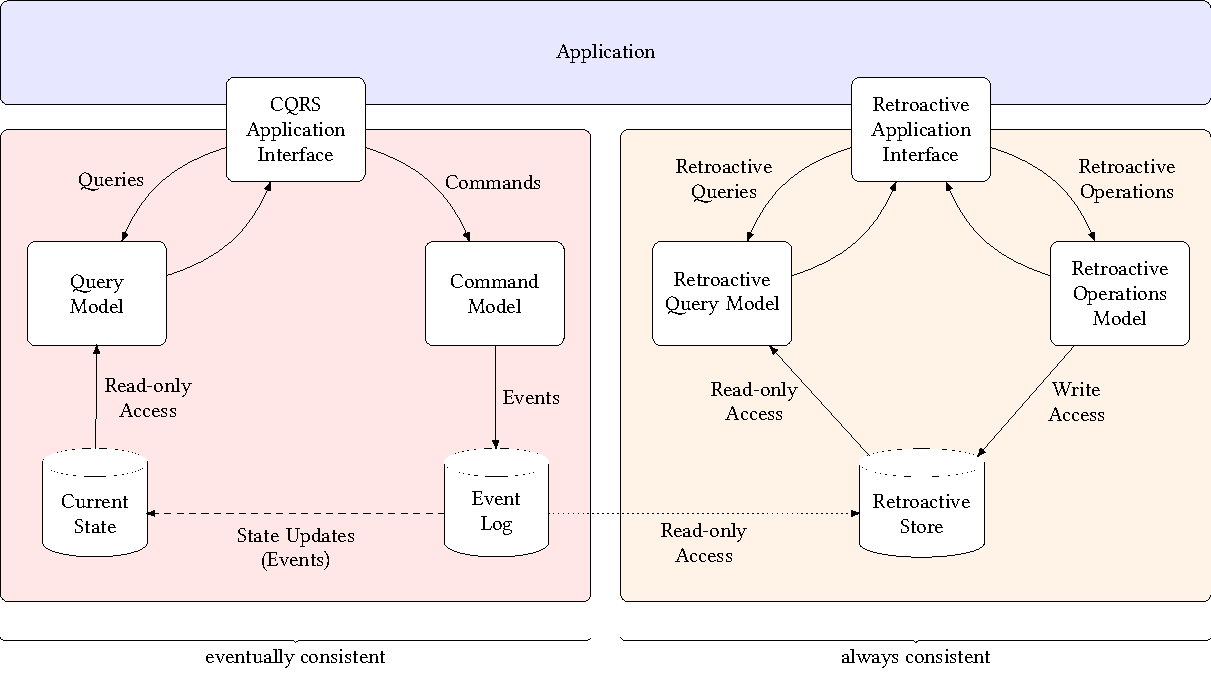
\includegraphics[height=6.7cm]{../illustrations/cqrs-focus-separate.pdf}
	\caption{
		The retroactive computing features are introduced as a plug-in.
		The dotted connection marks the only connection from the component to the 
		original model: the retroactive store needs access to the event log.
	}
	\label{fig:rc-separate}
\end{figure*}

The idea of CQRS is that commands and queries operate on separate models. As
detailed in Section \ref{sec:issues-ec}, this is well suited when building 
systems in which an eventually consistent behavior is inevitable, but not 
appropriate for our use cases of retroaction. 
Following our argumentation from Section \ref{sec:issues-ec}, we thus do 
\emph{not} apply CQRS for the retroactive computing features in the following 
architectures. Instead, we propose for retroactive operations and retroactive 
queries to both operate on the same data model. This way, the data model can 
enforce causality.

\begin{figure*}[t]
	\centering
	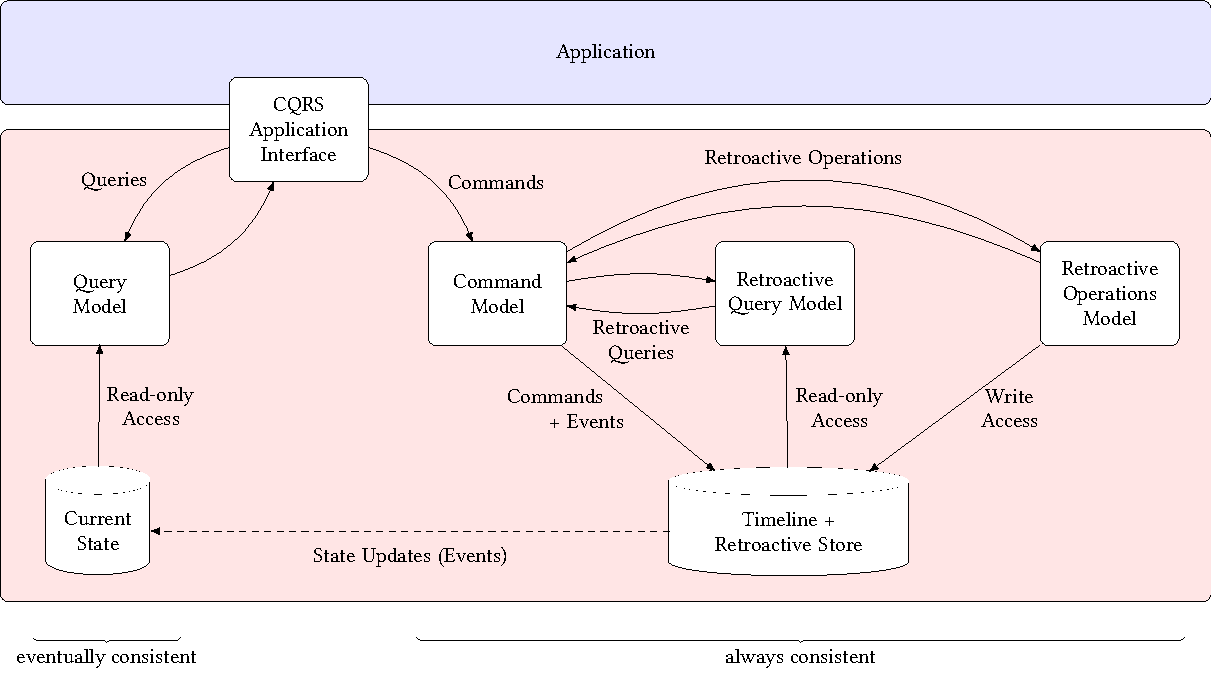
\includegraphics[height=6.7cm]{../illustrations/cqrs-focus-embedded2.pdf}
	\caption{
		This architecture design integrates the retroactive computing 
		capabilities into the ES+CQRS architecture in a more unified 
		approach. 
	}
	\label{fig:embedded}
\end{figure*}

\subsection{Plug-in Architecture}
\label{sec:arch:arch-plugin}
The first option which we describe introduces retroactive computing as an 
additional, separate component into an existing ES+CQRS system. The system 
is strictly event-sourced: commands are not persisted, solely events are 
sourced. Retroactive computing in this architecture takes place on a high 
level, in the application.
This is how CQRS is usually applied: The business logic resides within the 
high level application layer and commands merely hide implementation details 
of how commands are executed.
This architecture is depicted in Figure \ref{fig:rc-separate}.
%
The retroactive features can be accessed within the application -- which 
already has access to the CQRS API over a Retroactive API.
The application using the component can execute retroactive queries and 
operations over this API.
%
The results from retroactive queries and operations are returned back to the
application, which can then decide how to use them.
A ``Retroactive Store'' component holds all branches and their modifications in
relation to the timeline. The ``normal'' event log possesses an append-only 
semantics and may not be retroactively modified. Branches in the retroactive 
store, on the other hand, can be edited directly. Causality of retroactive 
operations and retroactive queries can be enforced by accessing the same model 
(marked as ``always consistent'' in the figure). 
This follows our ideas described for what-if questions in Section \ref{sec:issues-ec}.

We have created a prototypical implementation of this architecture with JavaScript 
as the scripting language for the underlying runtime engine and JSON as the 
data format for events and commands. The scenario implemented in our prototype 
is an online shop with retroactive capabilities.
The online shop exposes functionalities via a web service API (displayed as the 
``CQRS API'' in the figure).
Through this interface it is possible to add products to a cart or place orders.
Over the ``Retroactive API'' it is possible to invoke retroactive commands, such 
as calculating hypothetical discounts, if orders would have been executed as a
privilege customer. %with a certain customer privilege status.

\subsection{Unified Architecture}
\label{sec:arch:arch-unified}
A contrasting possibility to the described plug-in architecture, is to integrate 
retroactive computing as an integral part of the ES+CQRS architecture in a way 
that retroactive operations or retroactive queries can be invoked within commands.
Retroaction thus can be viewed as an integral part of the programming model. 
As in the plug-in architecture, causality of retroactive operations and 
retroactive queries is enforced in this architecture as well. 
This is achieved by accessing the same model (``always consistent'' in the figure).
The only way for the application to access retroactive capabilities is by 
issuing commands. It is not possible to access retroactive features directly 
from the query model.
%
In order for the application to query results of retroactive operations, an event 
needs to be appended to the log.
This is not ideal for all use cases, since the event is replicated to all query 
models. Especially in large systems with many replicated query models, this
might be an unnecessary overhead.
But this concept of persisting retroaction via events, resonates with the idea 
that state mutations are persisted and thus the state of a system can always be 
traced or rebuilt. 
There exists only one store in this architecture, it contains the timeline and 
its branches. 
%
A conceptual and prototypical implementation of this architecture is described 
in Chapter \ref{chp:programming}.

\subsection{Comparison}
Each architecture addresses a different layer of interaction with the retroactive 
capabilities. In the plug-in architecture, retroaction is added as an additional 
feature to a traditional CQRS architecture. Application commands can even be 
issued based upon retroactive insights. 
Though this should not have the consequence that the application creates its 
own commands by querying the retroactive store and issue application commands 
based upon the results. 
The idea behind CQRS for the application is to issue commands, but not to define 
commands. If this happens, %, this is no longer a CQRS architecture. Instead this 
this results in an architecture where commands (i.e. application logic) and state 
resides in multiple components.
Thus commands and state are not always persisted in the timeline. This breaks the 
traceability of a system and restoring arbitrary states is no longer possible.

In the unified architecture, on the other hand, application commands access 
retroactive features indirectly.
Retroaction is integrated into the programming model, which thus gains the 
ability to access and manipulate past states of objects and explore alternate 
states. This enables a retroactively expressive programming model and makes 
certain application commands and queries feasible, which are not possible 
otherwise (e.g. calculating a discount based on previous orders, in a 
\texttt{PlaceOrder} command).
A further advantage of this unified approach is that the access to retroactive
features happens in the same environment as the programming takes place.
This enables developers to use data structures, functions, and libraries from 
the program in the retroactive code.

Introducing retroactive computing as a plug-in requires no modifications to an 
existing CQRS architecture and can thus be advantageous when enhancing an 
existing architecture. There is only one connection from the plug-in to the 
original model: the plug-in needs access to the event log. The integration of 
retroactive computing as a core part of an ES+CQRS architecture, on the other 
hand, does not suit well with existing event-sourced systems, since it requires 
profound architectural modifications. 
Nevertheless, it yields more expressive commands and has possibilities which 
cannot be reached with a plug-in.

In the separate architecture, modifications to the event log are recorded in the 
retroactive store, but not in the event log. Restoring state based solely on the 
event log thus is no longer sufficient, the retroactive store needs to be rebuild 
as well. 
In the unified architecture, on the other hand, the commands using retroaction 
are sourced, as well as their resulting events. Retroaction is part of a command 
and results in events. Thus, the timeline always contains all retroactive 
operations ever applied -- it is still the only source of application history.

Retroactive operations can be quite costly, since they might require a lot of 
recomputations. In the plug-in, these costs arise only when retroactive operations 
are applied; otherwise they are not present and do not influence the performance
of the system. 
The unified architecture, however, imposes more costs to the overall system
performance, since commands need to be sourced and the effects of retroactive 
operations are replicated.
Furthermore, if a command in the unified architectures applies complex retroactive 
operations, the further execution of sequential commands is blocked. Thus, if a 
command starts with expensive retroactive calculations, the execution of subsequent 
commands halts. The eventually consistent semantics of commands and queries 
mitigates this issue, but it is still not ideal.

Many of the ideas introduced in this chapter only play out their full strength 
if an ES+CQRS system is built with them in mind from the ground up. For example, 
splitting the side effects from larger commands into individual commands for 
better control in replays is hard to do in existing systems.

\section{Summary}
In this chapter, we described a number of conceptual issues when utilizing 
retroaction in event-sourced systems. The two most pressing issues concern the 
dealing with side effects and issues of keeping a consistent timeline.
We illustrated that restraining direct editing operations to branches of
a timeline can prevent causality issues. Furthermore, it is possible to retain 
traceability and append-only behavior in event-sourced systems if results from 
retroaction are integrated back into the system as events.

In order to impose control over side effect afflicted commands in replay
scenarios, we discussed several possibilities and concluded the discussion
by introducing the idea of partial replays which require tracking causalities 
among events. If side effects are outsourced into separate, individual commands 
they can be partially reused or reinvoked.
The command and event primitives of event sourcing are an ideal match for 
imposing control over side effects. Through events, side effects can be 
recorded and re-used. Through the sourcing of commands, side effects can be 
reinvoked.

Next, we discussed a number of ideas for keeping a consistent timeline after a
retroactive modification. For this, we transferred ideas from time travel 
theory to retroaction in event-sourced systems. As correspondences to parallel 
universes we proposed to prohibit editing the own timeline and allow direct 
retroactive modifications only for branches.
Analogue to the  self-consistency principle, we proposed validation conditions 
and the replay (or removal) of causally related events. 
We examined, that validation conditions can only be imposed once the result 
of a command is clear, for which the command needs to be invoked.
This problem is especially challenging once the command yielded side effects,
which cannot be revoked.
%
Furthermore, this chapter contributed an overview on constraints and limitations 
of retroaction in event-sourced systems. We highlighted the central role of 
hidden causalities through real-world coupling or through side effects. Further 
limitations, which we identified, were the influence of causality violations, 
causally equivalent replays, and the semantics of commands which may annihilate
retroactive modifications. The performance of retroactive computations can be a 
further limiting factor.

Our conceptual considerations were concluded with the suggestion of architectural 
modifications (e.g. resolving the command/query segregation for retroaction) and 
the demonstration how different architectures can be used for enabling retroactive 
capabilities of event-sourced applications.
